Translater notre système, actuellement dans une situation de carrefour parfait, dans une situation de carrefour mal fait, est possible. Sous contrainte que nous disposions d’un plus grand nombre de senseurs, il serait envisageable de rendre un carrefour illogique plus optimisé. Prenons un exemple concret :

\begin{figure}[H]
    \begin{center}
        \frame{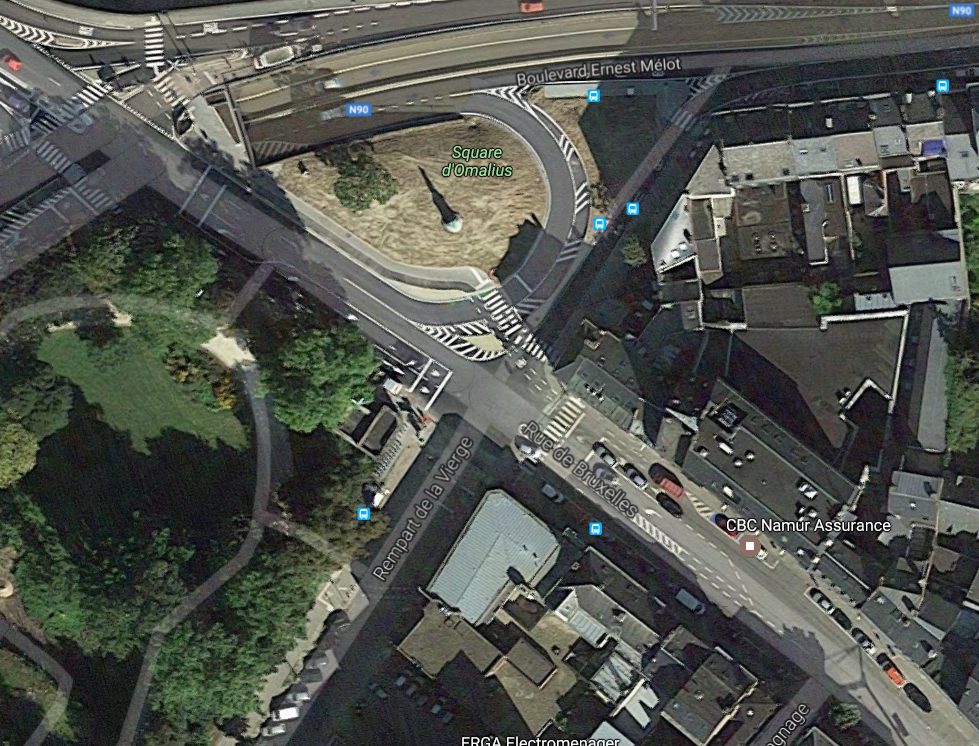
\includegraphics[width=\linewidth, height=\textheight,keepaspectratio]{img/application-realite}}

        \caption{Carrefour non loin des facultés de l'UNamur}
    \end{center}
\end{figure}
\vspace{-0.5cm}
Comme nous pouvons le constater, il y a des voies provenant d’un peu partout. La N90 permet deux entrées dans le carrefour : soit le long du parc Louise-Marie, soit par le Square d’Omalius après être passé sous le carrefour. Des véhicules proviennent également de la rue de Bruxelles, de l’Avenue des Combattants ainsi que du Rempart de la Vierge. A noter que les véhicules provenant de la N90 par le parc Louise-Marie peuvent tourner dans toutes les directions, alors que ceux provenant du Square d’Omalius sont obligés de se diriger vers l’Avenue des Combattants. Les véhicules venant du nord par la N90 et se dirigeant vers l’Avenue des Combattants, ainsi que ceux provenant de cette dernière et allant vers le sud par la N90 ne sont pas repris dans le carrefour, puisqu’ils doivent respecter le principe du “Cédez le passage”.\\

Notre solution repose sur le fait qu’une voie est prioritaire par rapport aux autres afin d’optimiser le passage sur la principale. Dans le cas présent, le gros de la circulation provient des deux entrées de la N90 et se dirige en grosse partie vers l’Avenue des Combattants. Il arrive également souvent qu’il n’y ai pas de voitures provenant de la Rue de Bruxelles et du Rempart de la Vierge, malgré que leur feu soit vert. Il serait dès lors possible d’avantager les deux entrées de la N90 par rapport aux autres voies. Tout comme sur notre maquette actuelle, des capteurs de présence nous permettraient d’évaluer la présence sur les autres axes, et de ne mettre au rouge les entrées de la N90 que lorsque des voitures se présentent sur ces axes.\\

De plus, de la même manière que nous pouvons conseiller aux usagers d’emprunter un chemin différent sur la maquette, nous pourrions ici détecter un embouteillage sur l’une des entrées de la N90 sur le carrefour, et conseiller aux automobilistes d’utiliser l’autre.\\

Au niveau du code, la translation vers ce carrefour serait très facile. Comme nous fonctionnons avec les acteurs, il suffirait de déclarer autant d’acteurs “Feu rouge” dans l’acteur “Carrefour” qu’il y a réellement de feux, et adapter les temps d’attente minimum de chaque axe.